\chapter{Finite Element Volume Method}
\label{chp:HFVMMethod}
In this chapter we introduce the notation for the numerical grids and then describe the second-order Finite Element Volume Method (FEVM) in detail.

A variety of numerical methods have been used to solve the Serre equations; from complete finite difference methods \cite{Cienfuegos-etal-2006-1217,El-etal-2006} and finite element methods \cite{Mitsotakis-etal-2014,Li-2014-169,Mitsotakis-etal-2017} to combinations of finite difference and finite volume methods \cite{Hank-etal-2010-2034,Zoppou-etal-2017}. Splitting techniques have also been employed, most commonly to split the Serre equations into their non-linear and dispersive parts; resulting in an elliptic operator for the dispersive part and the SWWE for the non-linear part \cite{Bradford-Sanders-2002-953,Dutykh-etal-2013-761,Filippini-etal-2016-381}. 

Numerical methods that make use of the conservation law form of the Serre equations \eqref{eqn:FullSerreCon} \cite{Hank-etal-2010-2034,Li-2014-169,Zoppou-etal-2017} are the most promising for the two dimensional Serre equations with variable bathymetry. The primary reason for this is that these methods are robust and extend well to unstructured meshes with complex geometries which are the meshes most commonly used for modelling physical scenarios. Secondly, to properly handle the elliptic operator produced by the non-linear and dispersive splitting requires overly restrictive assumptions about the smoothness of the physical quantities, particularly the water depth. 

I have developed an extension of the Finite Difference Volume Methods (FDVM) \cite{Hank-etal-2010-2034,Zoppou-etal-2017} that uses a finite element method in place of the finite difference method. This second-order FEVM which will be referred to as $\text{FEVM}_2$ was a main objective of the thesis; it consists of two main parts a Finite Element Method (FEM) to solve \eqref{defn:SerreEqnConservedQuantity1} and a Finite Volume Method (FVM) to solve \eqref{eqn:FullSerreCon} hence its name. Making use of these two methods results in a numerical method with a number of desirable properties. It is robust in the presence of steep gradients in the free surface \cite{Pitt-2018-61}, robust during the wetting and drying of beds and all the terms of the finite volume method can be calculated knowing only the quantities inside the cell. This last point indicates that this method is the ideal variant of the finite volume based methods \cite{Zoppou-etal-2017} to be extended to solve the two-dimensional Serre equations on unstructured meshes with parallelised code.
 
 
In addition to the $\text{FEVM}_2$, the first- and second-order FDVM of \citet{Hank-etal-2010-2034} and \citet{Zoppou-etal-2017} were reproduced. These methods will be referred to as $\text{FDVM}_1$ and $\text{FDVM}_2$ respectively. Furthermore the third-order $\text{FDVM}_3$ was implemented during my research. I have also reproduced the second-order naive finite difference method \cite{Pitt-J-2014} and the finite difference method of \citet{El-etal-2006}; which I refer to as $\mathcal{D}$ and $\mathcal{W}$ respectively. Descriptions of these methods have already been published \cite{Zoppou-etal-2017,Pitt-2018-61} and therefore, are omitted from the thesis.


\section{Notation for Numerical Grids}

In the $\text{FEVM}_2$, time and space will be discretised in different ways. Time is broken up into time levels separated by a constant duration $\Delta t$ and space is broken up into cells of constant width $\Delta x$. The FEVM can be extended to allow for varying $\Delta t$ and $\Delta x$ values, with this description restricted to the constant case for simplicity. The notation for time is quite simple; from an initial time $t^0$ we define the $n^{th}$ time level where $n \in \mathbb{N}$ to be
\begin{align*}
t^n &= t^0 + n \Delta t.
\end{align*}
The goal of $\text{FEVM}_2$ is to update the quantities at the current time level $t^n$ to the next time level $t^{n+1}$ by solving the equations. 

The notation for space is a bit more complicated; as we require definitions of multiple locations inside the cells. The cells are defined by their midpoints; which are given from a starting location $x_0$, so that the midpoint of the $j^{th}$ cell where $j \in \mathbb{N}$ is
\begin{align*}
x_j &= x_0 + j \Delta x.
\end{align*}
Other points inside the $j^{th}$ cell can be defined in relation to the midpoint so that 
\begin{align*}
x_{j + s} &= x_j + s \Delta x
\end{align*}
where $s \in \left[-\frac{1}{2} , \frac{1}{2}\right] \subset\mathbb{R}$, although for our purposes we restrict ourselves to rational values of $s$. Using this notation the $j^{th}$ cell spans $\left[x_{j -1/2},x_{j + 1/2}\right]$. These discretisations in space and time result in the grids displayed in Figure \ref{fig:NumericalGrid}.

\begin{figure}
	\centering
	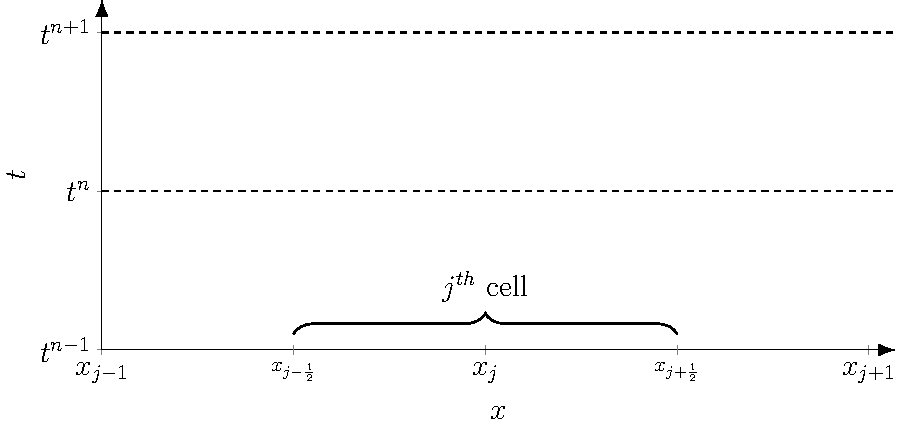
\includegraphics[width=0.8\textwidth]{./chp3/figures/Discretisation.pdf}
	\caption{Diagram of the time levels $t^{n-1}$, $t^n$ and $t^{n+1}$ at which the numerical solution of the Serre equations will be calculated. The $j^{th}$ cell with midpoint $x_{j}$ spanning $x_{j-1/2}$ to $x_{j+1/2}$ which is a volume of the FVM and an element of the FEM is also shown.}
	\label{fig:NumericalGrid}
\end{figure}

The temporal and spatial grid notation naturally extends to our quantities of interest, for example, for a general quantity $q$
\begin{equation*}
q^n_j = q(x_j ,t^n). 
\end{equation*}
These are the nodal values of $q$. Since the FEVM uses a FVM the cell averages of the quantities are also required. For each cell we define the average of a quantity at time level $t^n$ as
\begin{equation*}
\overline{q}_j^n = \frac{1}{\Delta x} \int_{x_{j-1/2}}^{x_{j+1/2}} q(x,t^n) \; dx
\end{equation*}
over the $j^{th}$ cell.

In the FEVM we reconstruct quantities at various points inside the cell using the adjacent cell average values. At the cell edges $x_{j\pm1/2}$, two reconstructions are possible from each of the neighbouring cells, we distinguish between the two possible reconstructions using superscripts. For example, for the cell edge $x_{j+1/2}$ and a general quantity $q$, there is the reconstructed value $q^-_{j+1/2}$ from the $j^{th}$ cell and the reconstructed value $q^+_{j+1/2}$ from the $(j+1)^{th}$ cell.

\section{Structure Overview}
\label{sec:StructOverview}
%define w,b
To describe the FEVM we first present an overview of the evolution step and then provide the details for each component. We begin our evolution step with all the cell averages for $h$, $w$ and $G$ at time $t^n$ and all the nodal values of $b$ being known. We write these as vectors from the starting $0^{th}$ to the final $m^{th}$ cell in the following way
\begin{align*} \overline{\vecn{q}}^n = \begin{bmatrix} \TM
\overline{q}_0^n \\\overline{q}_1^n \\ \vdots \\ \overline{q}_m^n \BM\end{bmatrix} & , & \vecn{b} = \begin{bmatrix} \TM
b_{0} \\ b_{1} \\ \vdots \\b_{m} \BM
\end{bmatrix} \\
\end{align*}
where $q$ is a generic quantity representing the vectors for $h$, $G$ and $w$. The evolution step proceeds by (i) reconstructing the quantities over the cell, (ii) calculating the fluid velocity, (iii) approximating the flux, (iv) approximating the source term, (v) updating the cell averages and then (vi) applying second-order time stepping.

\begin{enumerate}[(i)]
	\item Reconstruction: The locations for the reconstruction of all the quantities in the $j^{th}$ cell are displayed in Figure \ref{fig:ReconLocs}. For the $j^{th}$ cell the quantities $h$, $w$ and $G$ are reconstructed at $x_{j-1/2}$, $x_{j}$ and $x_{j+1/2}$ from their cell average values using the second-order reconstruction operators $\mathcal{R}^+_{j-1/2}$, $\mathcal{R}_{j}$ and $\mathcal{R}^-_{j+1/2}$ respectively. While the bed profile $b$ in the $j^{th}$ cell is reconstructed at $x_{j-1/2}$, $x_{j-1/6}$, $x_{j+1/6}$ and $x_{j+1/2}$ from its nodal values using the fourth-order reconstruction operators $\mathcal{B}_{j-1/2}$, $\mathcal{B}_{j-1/6}$, $\mathcal{B}_{j+1/6}$ and $\mathcal{B}_{j+1/2}$ respectively. 
	\begin{figure}
		\centering
		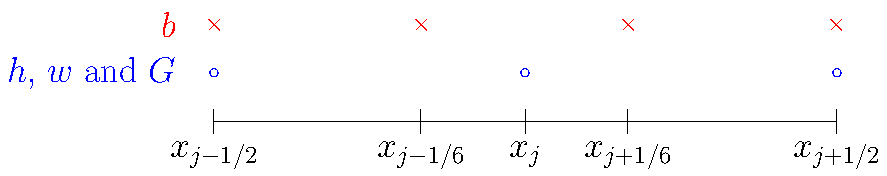
\includegraphics[width=0.8\textwidth]{./chp3/figures/FEVMRecon.pdf}
		\caption{The locations of the reconstructions for $h$, $w$, $G$ (\circlet{blue}) and $b$ (\crosst{red}) inside the $j^{th}$ cell.}
		\label{fig:ReconLocs}
	\end{figure}
	
	So that for a generic quantity $q$ representing $h$, $w$ and $G$ and the bed $b$ we have
	\begin{align*}
	&q^\pm_{j\pm 1/2} = \mathcal{R}^\pm_{j \pm1/2} \left(\overline{\vecn{q}}^n\right), &&b_{j\pm 1/2} = \mathcal{B}_{j\pm 1/2} \left(\vecn{b}\right),  \\
	&q_{j} = \mathcal{R}_{j} \left(\overline{\vecn{q}}^n\right), &&b_{j\pm 1/6} = \mathcal{B}_{j\pm 1/6}  \left(\vecn{b}\right).
	\end{align*}
	To keep the notation simple the time superscript is omitted from the reconstructed quantities.	This generates the vectors of these quantities reconstructed for every cell; $\vecn{\hat{h}}$, $\vecn{\hat{w}}$, $\vecn{\hat{G}}$ and $\vecn{\hat{b}}$ at time $t^n$ which are
	\begin{align*}\vecn{\hat{q}} = \begin{bmatrix} \TM
	q^+_{-1/2} \\ q_0 \\ q^-_{1/2} \\ \vdots  \\ q^-_{m+1/2} \BM \end{bmatrix} & , & \vecn{\hat{b}} = \begin{bmatrix} \TM
	b_{-1/2} \\ b_{-1/6} \\ b_{1/6}  \\b_{1/2}  \\ \vdots \\ b_{m+1/2} \BM
	\end{bmatrix}
	\end{align*}
	where $q$ is a generic quantity demonstrating these vectors for $h$, $w$ and $G$.	
	\item Fluid Velocity: The remaining unknown quantity, the horizontal velocity of the fluid column, $u$ is calculated at $x_{j-1/2}$, $x_j$ and $x_{j+1/2}$ in each cell by solving \eqref{defn:SerreEqnConservedQuantity1} with a second-order FEM. We denote the solution map of the FEM by $\mathcal{G}$, which takes $\vecn{\hat{h}}$, $\vecn{\hat{G}}$ and $\vecn{\hat{b}}$ as inputs. So that
	\begin{equation*}
	\vecn{\hat{u}} = 
	\begin{bmatrix} \TM	u_{-1/2} \\ u_0 \\ u_{1/2} \\ \vdots \\ u_{m+1/2} \BM
	\end{bmatrix} = \mathcal{G}\left( \vecn{\hat{h}}, \vecn{\hat{G}},\vecn{\hat{b}} \right).
	\end{equation*}
	\item Flux Across Cell Interfaces: We calculate the temporally averaged fluxes $F^n_{j-1/2}$ and $F^n_{j+1/2}$ across the cell boundaries $x_{j-1/2}$ and $x_{j+1/2}$ using $\mathcal{F}_{j-1/2}$ and $\mathcal{F}_{j+1/2}$, so that
		\begin{align*}	
		F^n_{j\pm 1/2} &=\mathcal{F}_{j\pm 1/2} \left( \vecn{\hat{h}}, \vecn{\hat{G}},\vecn{\hat{b}}, \vecn{\hat{u}}  \right).
		\end{align*}
	\item Source Terms: We calculate the source term contribution to the cell average of a quantity over a time step; $S^n_{j}$ with the operator $\mathcal{S}$
	\begin{equation*}	
	S^n_{j} =\mathcal{S}_{j} \left( \vecn{\hat{h}},\vecn{\hat{w}},\vecn{\hat{b}}, \vecn{\hat{u}}  \right).
	\end{equation*}
	\item Update Cell Averages: We update the cell average values from time $t^n$ to $t^{n+1}$ with a forward Euler approximation, resulting in a method that is second-order accurate in space and first-order in time.
	\item Second-Order SSP Runge-Kutta Method: We repeat steps (i)-(v) and use SSP Runge-Kutta time stepping to obtain $\overline{\vecn{h}}$ and $\overline{\vecn{G}}$ at $t^{n+1}$ with second-order accuracy in space and time.
\end{enumerate}


\subsection{Reconstruction}
\label{subsec:Reconstruction}
We now provide details for the reconstruction of $h$, $w$, $G$ and $b$ in the $j^{th}$ cell at the locations shown in Figure \ref{fig:ReconLocs}. For the purposes of the reconstruction we will assume that the mesh is structured. The reconstruction methods described here can be extended to unstructured meshes through generalisations of the interpolation techniques employed here \cite{Preneter-1975,atkinson-1978}. For $h$, $w$ and $G$ the reconstructions are performed from the cell averages. While $b$ is reconstructed from the nodal values. 

\subsubsection{Reconstruction of the $h$, $w$ and $G$}
We reconstruct $h$, $w$ and $G$ with piecewise linear functions over a cell from neighbouring cell averages. Since $h$, $w$ and $G$ use the same reconstruction operators we demonstrate them for a general quantity $q$. For the $j^{th}$ cell we reconstruct the values of $q$ at $x_{j-1/2} $, $x_{j} $ and $x_{j+1/2}$ in the following way
%cite someone 
\begin{subequations}
	\begin{align}
	q^+_{j-1/2} & = \mathcal{R}^+_{j-1/2} \left(\overline{\vecn{q}}\right) = \overline{q}_j - \dfrac{\Delta x}{2} d_j, \\
	q_{j} &= \mathcal{R}_{j} \left(\overline{\vecn{q}}\right) =\overline{q}_j ,\\
	q^-_{j+1/2} &= \mathcal{R}^-_{j+1/2} \left(\overline{\vecn{q}}\right) = \overline{q}_j + \dfrac{\Delta x}{2} d_j
	\end{align}
	\label{eqn:ReconforhwG}
\end{subequations}
where 
\begin{equation}
d_j = \text{minmod}\left(\theta \dfrac{\overline{q}_j -\overline{q}_{j-1} }{\Delta x}, \dfrac{\overline{q}_{j+1} -\overline{q}_{j-1} }{2\Delta x}, \theta\dfrac{\overline{q}_{j+1} -\overline{q}_{j} }{\Delta x}\right)
\label{eqn:slopehGrecon}
\end{equation}
with $\theta \in \left[1,2\right]$. The choice of the $\theta$ parameter changes the diffusion introduced by the reconstruction. When $\theta =1$ the reconstruction introduces the most diffusion and is equivalent to the minmod reconstruction \cite{Roe-1986-337}. When $\theta = 2$ the reconstruction introduces the least diffusion and is equivalent to the monotized central reconstruction \cite{VanLeer-1977-276}.

\begin{defn}
The minmod function
\begin{equation*}
\text{minmod}\left(a_0,a_1,\dots\right) := \left\lbrace \begin{array}{l l}
\min\left\lbrace a_i\right\rbrace & a_i > 0 \; \text{for all } i \\
\max\left\lbrace a_i\right\rbrace & a_i < 0  \; \text{for all } i \\
0 & \text{otherwise}\\
\end{array} \right.
\end{equation*}
takes a list of $a_i \in \mathbb{R}$. If all the inputs have the same sign then minmod returns the input with smallest absolute value, otherwise it returns zero. 
\end{defn}
The non-linear limiting used to calculate $d_j$ ensures that the reconstruction of $h$, $w$ and $G$ inside the cell is Total Variation Diminishing (TVD) \cite{Harten-1983-357}, hence it does not introduce non-physical oscillations. The TVD property of this reconstruction is achieved by constraining the slope $d_j$ to zero near local extrema, resulting in a piecewise constant reconstruction which is TVD. Away from local extrema $d_j$ will be the gradient with the smallest absolute value, making our reconstruction second-order accurate.

The reconstruction operator $\mathcal{R}_{j} $ is second-order accurate regardless of the presence of local extrema. This can be seen through the error analysis of the midpoint quadrature rule \cite{Davis-Rabinowitz-1984} for which we have that
\begin{equation}
\overline{q}^n_j = \frac{1}{\Delta x} \int_{x_{j-1/2}}^{x_{j+1/2}} q(x,t^n) \; dx = q_j^n + \mathcal{O}\left(\Delta x^2\right).
\end{equation}

\subsubsection{Reconstruction of the Bed Profile}
For the bed profile we require a reconstruction that is at least second-order accurate for $b$, $\partial b / \partial x$ and $\partial^2 b / \partial x^2$. To accomplish this $b$ is reconstructed with a cubic polynomial $C_j(x)$ centred around $x_j$
\begin{equation*}
C_j(x) = c_0 \left(x - x_j\right)^3 + c_1 \left(x - x_j\right)^2 + c_2 \left(x - x_j\right) + c_3.
\label{eqn:cubicforbedrecon}
\end{equation*}

By forcing $C_j(x)$ to pass through the nodal values $b_{j-2}$, $b_{j-1}$, $b_{j+1}$ and $b_{j+2}$ we get
\begin{equation*}
\begin{bmatrix}
\TM -8\Delta x^3 & 4\Delta x^2  & -2\Delta x & 1\\
-\Delta x^3 & \Delta x^2  &-\Delta x & 1\\
\Delta x^3 & \Delta x^2  & \Delta x & 1\\
8\Delta x^3 & 4\Delta x^2  & 2\Delta x & 1 \BM 
\end{bmatrix}
\begin{bmatrix}
 \TM c_0 \\ c_1 \\ c_2 \\ c_3  \BM\end{bmatrix} =  \begin{bmatrix}
 \TM b_{j-2} \\ b_{j-1}\\ b_{j+1} \\ b_{j+2} \BM
\end{bmatrix}.
\end{equation*}
Solving this we get the polynomial coefficients for $C_j(x)$
\begin{align*}
c_0 &=  \dfrac{-b_{j-2} + 2b_{j-1} - 2 b_{j+1} + b_{j+2}}{12 \Delta x^3},\\ \\
c_1 &=  \dfrac{b_{j-2} - b_{j-1} - b_{j+1} + b_{j+2}}{6 \Delta x^2},\\ \\
c_2 &=  \dfrac{b_{j-2} - 8b_{j-1} + 8 b_{j+1} - b_{j+2}}{12 \Delta x},\\ \\
c_3 &=  \dfrac{-b_{j-2}  + 4b_{j-1} + 4 b_{j+1} - b_{j+2}}{6}.
\end{align*}
We require a continuous bed profile and so we average the two reconstructions at the cell edge from the adjacent cells. Therefore, our reconstruction of the bed profile in the $j^{th}$ cell is the cubic which takes these values
\begin{align*}
b_{j-1/2} &=  \mathcal{B}_{j-1/2}\left(\vecn{b}\right) =  \frac{1}{2}\left( C_j(x_{j-1/2}) + C_{j-1}(x_{j-1/2})\right),\\
b_{j-1/6} &=  \mathcal{B}_{j-1/6}\left(\vecn{b}\right) =  C_j(x_{j-1/6}),\\
b_{j+1/6} &=  \mathcal{B}_{j+1/6}\left(\vecn{b}\right) =  C_j(x_{j+1/6}),\\
b_{j+1/2} &=  \mathcal{B}_{j+1/2}\left(\vecn{b}\right) =  \frac{1}{2}\left( C_j(x_{j+1/2}) + C_{j+1}(x_{j+1/2})\right).
\end{align*}


\subsection{Fluid Velocity}
\label{subsec:FluidVelocity}
In the FEVM we solve for the primitive variable $u$ given $h$, $G$ and $b$ using a finite element approximation to \eqref{defn:SerreEqnConservedQuantity1}. For the FEM we begin with the weak form of \eqref{defn:SerreEqnConservedQuantity1} with test function $v$ over the spatial domain $\Omega$ which is 

\begin{equation*}
	\int_{\Omega } G v \; dx =  \int_{\Omega } uh \left(1 + \frac{\partial h}{\partial x}\frac{\partial b}{\partial x} + \frac{1}{2}h\frac{\partial^2 b}{\partial x^2} +  \left[\frac{\partial b}{\partial x}\right]^2 \right) v - \frac{\partial}{\partial x}\left(\frac{1}{3}h^3  \frac{\partial {u}}{\partial x}\right) v \; dx.
\end{equation*}

Integrating by parts with zero Dirichlet boundary conditions we get
\begin{multline}
\int_{\Omega } G v \; dx = \int_{\Omega } uh \left(1 + \left[\frac{\partial b}{\partial x}\right]^2 \right) v \; dx +  \int_{\Omega } \frac{1}{3}h^3  \frac{\partial {u}}{\partial x} \frac{\partial v}{\partial x} \; dx  \\ - 
\int_{\Omega }   \frac{1}{2} u h^2\frac{\partial b}{\partial x}  \frac{\partial v }{\partial x}\; dx - 
\int_{\Omega }   \frac{1}{2}h^2\frac{\partial b}{\partial x}  \frac{\partial u }{\partial x}v \; dx.
\label{eqn:WeakFormDomain}
\end{multline}
By assuming that time is fixed so that all the functions only vary in space, this formulation implies that by ensuring that $G$, $h$, $b$ and $\partial b / \partial x$ have finite integrals over $\Omega$, then $u$ and $\partial u / \partial x$ must have finite integrals as well. Since we require $\partial u / \partial x$ to be well defined to approximate the fluxes and the source term \eqref{eqn:FullSerreCon} and thus have finite integrals we will assume that for each time $t$ that $h,G \in \mathbb{L}^2(\Omega)$ and $b \in\mathbb{W}^{1,2}(\Omega)$ so that $u \in \mathbb{W}^{1,2}(\Omega)$. See Appendix \ref{app:FEMIntegrals} for a precise definition of $\mathbb{L}^2(\Omega)$ and $\mathbb{W}^{1,2}(\Omega)$.

We simplify \eqref{eqn:WeakFormDomain} by performing the integration over the cells and then summing the integrals together to get the equation for the entire domain
\begin{multline}
\label{eq:elementwiseint}
 \sum_{j} \Bigg(  \int_{x_{j-1/2} }^{{x_{j+1/2}}} \Bigg[  \left( uh \left(1 + \left[\frac{\partial b}{\partial x}\right]^2 \right)  - \frac{1}{2}h^2\frac{\partial b}{\partial x}  \frac{\partial u }{\partial x}  -  G \right) v   \\ +  \left(\frac{1}{3}h^3  \frac{\partial {u}}{\partial x}    -     \frac{1}{2} uh^2\frac{\partial b}{\partial x}    \right) \frac{\partial v }{\partial x} \Bigg]dx \Bigg)  = 0
\end{multline}
which holds for all test functions $v$. The next step is to replace the functions for the quantities $h$, $G$, $b$ and $u$ with their corresponding basis function approximations. 

\subsubsection{Basis Function Approximations}
%mention what these basis functions ARE!@!!!!!
For $h$ and $G$ we use the basis functions $\psi$ \eqref{eqn:App1:PsiDef} which are linear inside a cell and zero elsewhere and so are not continuous as shown in Figure \ref{fig:P1DiscBasis}. This is consistent with our reconstruction which is second-order accurate inside the cell and possesses discontinuities at the cell edges. Since these basis functions are in $\mathbb{L}^2(\Omega)$ our basis function approximations to $h$ and $G$ are in the appropriate function space.
\begin{figure}
	\centering
	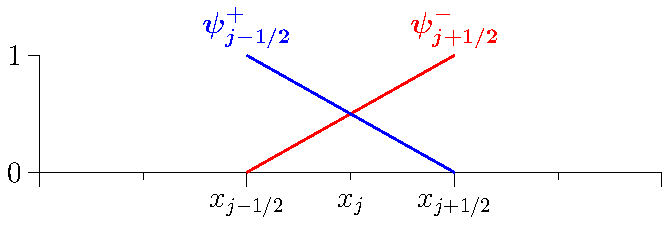
\includegraphics[width=0.8\textwidth]{./chp3/figures/P1.pdf}
	\caption{Support of the discontinuous linear basis functions $\psi$ over a cell.}
	\label{fig:P1DiscBasis}
\end{figure}

From the basis functions $\psi$ we have the following representation for $h$ and $G$ in our FEM written for the generic quantity $q$
\begin{align}
\label{eqn:FEapproxtohG}
q &= \sum_j \left( q^+_{j-1/2}\psi^+_{j-1/2}  + q^-_{j+1/2}\psi^-_{j+1/2}, \right).
\end{align}

To calculate the flux and source terms in \eqref{eqn:Serreconsconmom} we require a locally  calculated second-order accurate approximation to the first derivative of $u$. To do this we require a quadratic representation of $u$ in each cell and since we desire $u\in\mathbb{W}^{1,2}(\Omega)$, this representation will be continuous across the cell edges $x_{j \pm 1/2}$. Therefore, we use the continuous quadratic basis functions $\phi_{j\pm1/2} $ and $\phi_{j} $ \eqref{eqn:App1:PhiDef} depicted in Figure \ref{fig:P2ContBasis}.
\begin{figure}
	\centering
	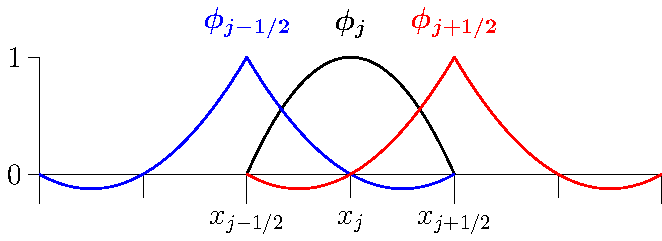
\includegraphics[width=0.8\textwidth]{./chp3/figures/P2.pdf}
	\caption{Support of the continuous piecewise quadratic basis functions $\phi$ over a cell.}
	\label{fig:P2ContBasis}
\end{figure}

From the basis functions $\phi$ our basis function approximation to $u$ is
\begin{equation}
u = u_{-1/2}\phi_{-1/2} + \sum_j \left( u_{j}\phi_{j} + u_{j+1/2}\phi_{j+1/2} \right).
\label{eqn:FEapproxtou}
\end{equation}

For the source term of the evolution of $G$ equation \eqref{eqn:Serreconsconmom} we require a local approximation to the second derivative of the bed that is also second-order accurate. To allow for an appropriate second derivative of the bed profile, $b$ must be a member of $\mathbb{W}^{2,2}(\Omega)$ which is smoother than required by \eqref{eqn:WeakFormDomain}. We choose the cubic basis functions $\gamma$ \eqref{eqn:App1:GamDef} which are continuous across the cell edges, as the bed profile will be continuous. These basis functions are shown in Figure \ref{fig:P3ContBasis} and from them we get our basis function approximation to $b$
\begin{figure}
	\centering
	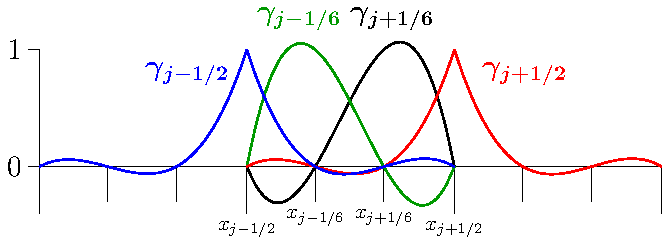
\includegraphics[width=0.8\textwidth]{./chp3/figures/P3.pdf}
	\caption{Support of the continuous piecewise cubic basis functions $\gamma$ over a cell.}
	\label{fig:P3ContBasis}
\end{figure}
\begin{equation}
b = b_{-1/2}\gamma_{-1/2} +  \sum_j \left(b_{j-1/6}\gamma_{j-1/6}  + b_{j+1/6}\gamma_{j+1/6} + b_{j+1/2}\gamma_{j+1/2} \right).
\label{eqn:FEapproxtob}
\end{equation}

\subsubsection{Calculation of Element-wise Matrices}
The integral equation \eqref{eq:elementwiseint} holds for all $v$. However, since our solution space has the basis functions $\phi$ it is sufficient to satisfy \eqref{eq:elementwiseint} for all $\phi$ to generate the solution. Since only the basis functions $\phi_{j-1/2}$, $\phi_{j}$ and $\phi_{j+1/2}$ are non-zero over the $j^{th}$ cell we can calculate the $j^{th}$ term in the sum \eqref{eq:elementwiseint} like so
\begin{multline}
\int_{x_{j-1/2} }^{{x_{j+1/2}}} \Bigg(  \left[ uh \left(1  +  \left[\frac{\partial b}{\partial x}\right]^2 \right)  - \frac{1}{2}h^2\frac{\partial b}{\partial x}  \frac{\partial u }{\partial x}  -  G \right] \begin{bmatrix} \TM
\phi_{j-1/2}\\\phi_j \\\phi_{j+1/2} \BM\end{bmatrix}   \\ +  \left[ \frac{1}{3}h^3  \frac{\partial {u}}{\partial x}    -     \frac{1}{2}h^2\frac{\partial b}{\partial x} u    \right] \frac{\partial}{\partial x}\left(\begin{bmatrix} \TM
\phi_{j-1/2}\\\phi_j \\\phi_{j+1/2}  \BM
\end{bmatrix} \right) \Bigg)dx
\label{eqn:WeakFormElemXspace}
\end{multline}
where we use our finite element approximations for $h$ \eqref{eqn:FEapproxtohG}, $G$ \eqref{eqn:FEapproxtohG}, $u$ \eqref{eqn:FEapproxtou} and $b$ \eqref{eqn:FEapproxtob}. This integral can be generalised by moving to the natural reference $\xi$-space, as the basis functions which are non-zero in one element are just translations of the non-zero basis functions in another element. The mapping from the $x$-space to the $\xi$-space is
\begin{equation*}
x = x_j + \xi \frac{\Delta x}{2}.
\end{equation*}
Therefore, the $j^{th}$ cell $\left[x_{j-1/2}, x_{j+1/2}\right]$ gets mapped to $\left[-1,1\right]$ in the $\xi$-space. Making the change of variables from $x$ to $\xi$ in \eqref{eqn:WeakFormElemXspace} we get
\begin{multline*}
\frac{\Delta x}{2}\int_{-1 }^{1} \Bigg( \left[ uh \left(1 + \frac{4}{\Delta x^2} \left[\frac{\partial b}{\partial \xi}\right]^2 \right)  - \frac{2}{\Delta x^2} h^2 \frac{\partial b}{\partial \xi}  \frac{\partial u }{\partial \xi}  -  G \right] \begin{bmatrix} \TM
\phi_{j-1/2}\\\phi_j \\\phi_{j+1/2} \BM
\end{bmatrix}   \\ + \frac{4}{\Delta x^2} \left[\frac{1}{3}h^3 \frac{\partial {u}}{\partial \xi}    -     \frac{1}{2}h^2 \frac{\partial b}{\partial \xi} u    \right] \frac{\partial}{\partial \xi}\left(\begin{bmatrix} \TM
\phi_{j-1/2}\\\phi_j \\\phi_{j+1/2} \BM
\end{bmatrix} \right) \Bigg)d\xi.
\end{multline*}

We will demonstrate the rest of the process for the $uh$ term as an example with the remaining integrals provided \href{https://sites.google.com/view/jordanpitt/phd-thesis-resources/finite-element-integrals}{\color{blue}\underline{online}} (https://sites.google.com/view/jordanpitt/phd-thesis-resources/finite-element-integrals).
The $uh$ term is 
\begin{equation*}
\frac{\Delta x}{2}\int_{-1 }^{1} uh \begin{bmatrix} \TM
\phi_{j-1/2}\\\phi_j \\\phi_{j+1/2} \BM
\end{bmatrix} d\xi.
\end{equation*}
Since the integral is computed over $\left[-1,1\right]$, there are only a few non-zero contributions from the finite element approximations to $h$ and $u$, so $uh$ term becomes
\begin{multline*}
\frac{\Delta x}{2}\int_{-1 }^{1}  \Bigg( \left(u_{j-1/2}\phi_{j-1/2} + u_{j}\phi_{j} + u_{j+1/2}\phi_{j+1/2}\right) \\ \times\left(h^+_{j-1/2}\psi^+_{j-1/2}  + h^-_{j+1/2}\psi^-_{j+1/2}\right) \begin{bmatrix} \TM
\phi_{j-1/2}\\\phi_j \\\phi_{j+1/2} \BM
\end{bmatrix} \Bigg) d\xi\\
=\frac{\Delta x}{2}\Bigg( h^+_{j-1/2} \int_{-1 }^{1} \psi^+_{j-1/2}  \begin{bmatrix} \TM
\phi_{j-1/2} \phi_{j-1/2} & \phi_{j}  \phi_{j-1/2}  & \phi_{j+1/2} \phi_{j-1/2}\\\phi_{j-1/2} \phi_{j} & \phi_{j} \phi_{j} &  \phi_{j + 1/2} \phi_{j}\\\phi_{j+1/2} \phi_{j-1/2} &  \phi_{j+1/2} \phi_{j} & \phi_{j+1/2} \phi_{j+1/2} \BM
\end{bmatrix} d\xi  \\ +  h^-_{j+1/2}\int_{-1 }^{1} \psi^-_{j+1/2} \begin{bmatrix} \TM
\phi_{j-1/2} \phi_{j-1/2} & \phi_{j}  \phi_{j-1/2}  & \phi_{j+1/2} \phi_{j-1/2}\\\phi_{j-1/2} \phi_{j} & \phi_{j} \phi_{j} &  \phi_{j + 1/2} \phi_{j}\\\phi_{j+1/2} \phi_{j-1/2} &  \phi_{j+1/2} \phi_{j} & \phi_{j+1/2} \phi_{j+1/2} \BM
\end{bmatrix} d\xi \Bigg)  \begin{bmatrix} \TM
u_{j-1/2}\\u_j \\u _{j+1/2} \BM
\end{bmatrix}.
\end{multline*}

Calculating the integrals of all the basis function combinations we get

\begin{multline*}
\frac{\Delta x}{2}\int_{-1 }^{1}  uh \begin{bmatrix} \TM
\phi_{j-1/2}\\\phi_j \\\phi_{j+1/2} \BM
\end{bmatrix} d\xi =  \\ \frac{\Delta x}{60}  \begin{bmatrix} \TM
7 h^+_{j-1/2} + h^-_{j+1/2} & 4 h^+_{j-1/2}   & - h^+_{j-1/2} - h^-_{j+1/2}\\ 4 h^+_{j-1/2} & 16 h^+_{j-1/2} + 16 h^-_{j+1/2}& 4 h^-_{j+1/2}\\ - h^+_{j-1/2} - h^-_{j+1/2} &  4 h^-_{j+1/2} &  h^+_{j-1/2} + 7 h^-_{j+1/2} \BM
\end{bmatrix}  \begin{bmatrix} \TM
u_{j-1/2}\\u_j \\u _{j+1/2} \BM
\end{bmatrix}.
%\label{eqn:FEMutermexample}
\end{multline*}

\subsubsection{Assembly of the Global Matrix}
By combining all the matrices generated by the integral of each of the $u$ terms we get the contribution of the $j^{th}$ cell to the stiffness matrix $\matr{A}_j$. Likewise all the integrals of the remaining term $Gv$ in \eqref{eq:elementwiseint} generate the element wise vector $\vecn{g}_{j}$. These element wise matrices and vectors are then assembled into the global stiffness matrix $\matr{A}$ and the global right hand-side term $\vecn{g}$ thus \eqref{eq:elementwiseint} is rewritten as
\begin{equation}
\label{eqn:FEMElemMatrixJ}
 \matr{A} \vecn{\hat{u}} = \vecn{g}.
\end{equation}
This is a penta-diagonal matrix equation which can be solved by direct banded matrix solution techniques such as those of \citet{NumRecC-1996} to obtain
\begin{equation}
\vecn{\hat{u}} =\mathcal{G}\left( \vecn{\hat{h}}, \vecn{\hat{G}},\vecn{\hat{b}} \right) =   \matr{A}^{-1}\vecn{g}
\label{eqn:usolvefromGhb}
\end{equation}
as desired.
\subsection{Flux Across the Cell Interfaces}

We use the method of \citet{Kurganov-etal-2001-707} to calculate the flux across a cell interface. This method was employed because it can handle discontinuities across the cell boundary and only requires an estimate of the maximum and minimum wave speeds. This is precisely the situation for the Serre equations which do not have a known expression for the characteristics but do possess estimates on the maximum and minimum wave speeds \eqref{eqn:WaveVelocitiesBound}.

Only the calculation of the flux term $F_{j+1/2}$ is demonstrated as the process to calculate the flux term $F_{j-1/2}$ is identical but with different cells. For a general quantity $q$ the approximation of the flux term given by \citet{Kurganov-etal-2001-707} is
\begin{equation}\label{eqn:HLL_flux}
F_{j+\frac{1}{2}} = \dfrac{a^+_{j+\frac{1}{2}} f\left(q^-_{j+\frac{1}{2}}\right) - a^-_{j+\frac{1}{2}} f\left(q^+_{j+\frac{1}{2}}\right)}{a^+_{j+\frac{1}{2}} - a^-_{j+\frac{1}{2}}}  + \dfrac{a^+_{j+\frac{1}{2}} \, a^-_{j+\frac{1}{2}}}{a^+_{j+\frac{1}{2}} - a^-_{j+\frac{1}{2}}} \left(  q^+_{j+\frac{1}{2}} - q^-_{j+\frac{1}{2}} \right)
\end{equation}
where $a^+_{j+\frac{1}{2}}$ and $a^-_{j+\frac{1}{2}}$ are given by bounds on the wave speed. Applying the wave speed bounds \eqref{eqn:WaveVelocitiesBound} we obtain

\begin{align}
a^-_{j+\frac{1}{2}} &= \min\left\lbrace 0\;,\;  u^-_{j + 1/2} - \sqrt{g h^-_{j + 1/2}}  \;,\;u^+_{j + 1/2} - \sqrt{g h^+_{j + 1/2}} \right\rbrace  ,\\
a^+_{j+\frac{1}{2}} &= \max\left\lbrace 0 \;,\;  u^-_{j + 1/2} + \sqrt{g h^-_{j + 1/2}}  \;,\;u^+_{j + 1/2} + \sqrt{g h^+_{j + 1/2}} \right\rbrace .
\label{eqn:WaveSpeedBoundsFluxApprox}
\end{align}

The flux functions $f(q^-_{j+\frac{1}{2}})$ and $f(q^+_{j+\frac{1}{2}})$ across the cell edge $x_{j+1/2}$ are evaluated using the reconstructed values $q^-_{j+\frac{1}{2}}$ from the $j^{th}$ cell and $q^+_{j+\frac{1}{2}}$ from the $(j+1)^{th}$ cell. From the continuity equation \eqref{eqn:FullSerreConMass} we have
\begin{align*}
f\left(h^\pm_{j+\frac{1}{2}}\right) &= u^\pm_{j + 1/2}  h^\pm_{j + 1/2}.
\end{align*}

For the evolution of $G$ equation \eqref{eqn:Serreconsconmom} we have 
\begin{align}
f\left(G^\pm_{j+\frac{1}{2}}\right) &=  u^\pm_{j + 1/2} G^\pm_{j + 1/2}  + \frac{g}{2}\left(h^\pm_{j + 1/2} \right)^2 - \frac{2}{3}\left(h^\pm_{j + 1/2}\right)^3 \left[\left(\frac{\partial {u}}{\partial x} \right)^\pm_{j + 1/2} \right]^2 \nonumber\\ &+ \left(h^\pm_{j + 1/2}\right)^2 u^\pm_{j + 1/2} \left(\frac{\partial {u}}{\partial x} \right)^\pm_{j + 1/2} \left(\frac{\partial b}{\partial x} \right)^\pm_{j + 1/2} .
\label{eqn:FluxIrrotNum}
\end{align}

The quantities $h^+_{j - 1/2}$, $h^-_{j + 1/2}$, $G^+_{j - 1/2}$ and $G^-_{j + 1/2}$ were calculated during the reconstruction and the FEM provided $u^\pm_{j+1/2} = u_{j+1/2}$ as $u$ is continuous across the cell boundaries.

\subsubsection{Calculation of Derivatives}
Approximations to $\left(\dfrac{\partial {b}}{\partial x} \right)^\pm_{j + 1/2}$ and $\left(\dfrac{\partial {u}}{\partial x} \right)^\pm_{j + 1/2}$ are now required to calculate the flux \eqref{eqn:FluxIrrotNum}. To calculate these derivatives in $u$ and $b$ we use the basis function approximation to these quantities in the FEM to define the reconstruction polynomial of these quantities over a cell. For $u$ we have the quadratic
	\begin{equation}
	P^u_j(x) = p^u_0 \left(x - x_j\right)^2 + p^u_1 \left(x - x_j\right) + p^u_2
	\label{eqn:Polyforucell}
	\end{equation}
that passes through $u_{j-1/2}$, $u_j$ and $u_{j+1/2}$. While for $b$ we have the cubic
	\begin{equation}
	P^b_j(x) = p^b_0 \left(x - x_j\right)^3 + p^b_1 \left(x - x_j\right)^2 + p^b_2 \left(x - x_j\right)  + p^b_3
	\label{eqn:Polyforbcell}
	\end{equation}
that passes through $b_{j-1/2}$, $b_{j-1/6}$, $b_{j+1/6}$ and $b_{j+1/2}$. Because the cell edge values were averaged during the reconstruction of the bed, $P^b_j(x)$ will be different from $C_j(x)$.

For $P^u_j(x)$ we obtain the coefficients
\begin{align*}
p^u_0 &=  \dfrac{u_{j-1/2} - 2u_j + u_{j+1/2}}{2 \Delta x^2},\\
p^u_1 &=  \dfrac{-u_{j-1/2} + u_{j+1/2}}{\Delta x},\\
p^u_2 &=  u_j.
\end{align*}
While for $P^b_j(x)$ the coefficients are
\begin{align*}
p^b_0 &=  \dfrac{-9b_{j-1/2} + 27b_{j-1/6} - 27 b_{j+1/6} + 9b_{j+1/2}}{2 \Delta x^3},\\ \\
p^b_0 &=  \dfrac{9b_{j-1/2} - 9b_{j-1/6} - 9b_{j+1/6} + 9b_{j+1/2}}{4 \Delta x^2},\\ \\ 
p^b_0 &=  \dfrac{b_{j-1/2} - 27b_{j-1/6} + 27 b_{j+1/6} - b_{j+1/2}}{8 \Delta x},\\\\
p^b_0 &=  \dfrac{-b_{j-1/2}  + 9b_{j-1/6} + 9 b_{j+1/6} - b_{j+1/2}}{16}.
\end{align*}
Taking the derivative of the polynomials \eqref{eqn:Polyforucell} and \eqref{eqn:Polyforbcell} we get
	\begin{align*}
	\frac{\partial }{\partial x}P^u_j(x) &= 2p^u_0 \left(x - x_j\right) + p^u_1, \\
	\frac{\partial }{\partial x}P^b_j(x) &= 3p^b_0 \left(x - x_j\right)^2 + 2p^b_1 \left(x - x_j\right) + p^b_2.
	\end{align*}
This gives a second-order approximation to the derivative of $u$ and $b$ at $x_{j+1/2}$ for the $j^{th}$ cell. The process for the $(j+1)^{th}$ cell is the same and we get 
	\begin{align*}
	\left(\dfrac{\partial {u}}{\partial x} \right)^-_{j + 1/2} &= \frac{\partial }{\partial x}P^u_j(x_{j+1/2}),  \\
	\left(\dfrac{\partial {u}}{\partial x} \right)^+_{j + 1/2} &= \frac{\partial }{\partial x}P^u_{j+1}(x_{j+1/2}),  \\
	\left(\dfrac{\partial {b}}{\partial x} \right)^-_{j + 1/2} &= \frac{\partial }{\partial x}P^b_j(x_{j+1/2}), \\
	\left(\dfrac{\partial {b}}{\partial x} \right)^+_{j + 1/2} &= \frac{\partial }{\partial x}P^b_{j+1}(x_{j+1/2}). 	\end{align*}

Therefore, we possess all the terms needed to calculate the approximation to the flux \eqref{eqn:HLL_flux} for $h$ and $G$, as desired. However, to ensure that the FEVM is well-balanced and recovers the lake at rest steady state solution, these fluxes must be modified.

\subsubsection{Well-Balancing Modification to Flux Approximation}
To recover the lake at rest steady state solution we follow the work of \citet{Klein-etal-2004-2050}, who accomplished this for the SWWE. Previously, we demonstrated that this process can be extended to the Serre equations \cite{Pitt-J-2014}. To enforce well-balancing the reconstruction of $h$ is modified at the cell edges in the following way.

First calculate
\begin{align}
\dot{b}^-_{j+1/2} = w^-_{j+1/2} - h^-_{j+1/2} &, &\dot{b}^+_{j+1/2} = w^+_{j+1/2} - h^+_{j+1/2}.
\label{eqn:BedReDefWmH}
\end{align}
Find the maximum
\begin{align*}
\ddot{b}_{j+1/2} = \max\left\lbrace\dot{b}^-_{j+1/2} , \dot{b}^+_{j+1/2} \right\rbrace
\end{align*}
then define
\begin{subequations}
\begin{align}
\ddot{h}^-_{j+1/2} &= \max\left\lbrace 0, w^-_{j+1/2} - \ddot{b}_{j+1/2}  \right\rbrace, \\  \ddot{h}^+_{j+1/2} &= \max\left\lbrace 0, w^+_{j+1/2} - \ddot{b}_{j+1/2} \right\rbrace.
\end{align}
\label{eqn:ModifiedHValue}
\end{subequations}
This generates the vector $\vecn{\ddot{h}}$
\begin{equation*}
\vecn{\ddot{h}}= \begin{bmatrix} \TM
\ddot{h}^+_{-1/2} \\ h_0 \\ \ddot{h}^-_{1/2} \\ \vdots  \\ \ddot{h}^-_{m + 1/2}  \BM \end{bmatrix}
\end{equation*}
which we use to calculate the flux term $F_{j+1/2}$ in \eqref{eqn:HLL_flux} for $h$ and $G$ instead of $\vecn{\hat{h}}$. Applying the same process but with different cells we obtain $F_{j-1/2}$ and we have
\begin{align*}	
F^n_{j\pm 1/2} &=\mathcal{F}_{j\pm1/2} \left(\vecn{\ddot{h}}, \vecn{\hat{G}},\vecn{\hat{b}}, \vecn{\hat{u}}  \right).
\end{align*}
for the evolution of $h$ and $G$ equations as desired.

\subsection{Source Terms}
To evolve the Serre equations \eqref{eqn:FullSerreCon}, we require an approximation to the source term at the cell centre $x_j$ which we denote as $S_j$. Equation \eqref{eqn:FullSerreConMass} has no source term, therefore we only present the calculation of the source term for equation \eqref{eqn:Serreconsconmom}.

Following the work of \citet{Klein-etal-2004-2050} to produce a well-balanced method, we split our approximation to $S^n_j$ into the centred source term $S_{ci}$ and the corrective interface source terms $S^{-}_{j + \frac{1}{2}}$ and $S^{+}_{j + \frac{1}{2}}$
\begin{equation*}
S^n_j =  S^{-}_{j + \frac{1}{2}} + \Delta x S_{ci} + S^{+}_{j - \frac{1}{2}}.
\end{equation*}
Where $S_{ci}$ is the naive source term approximation and $S^{-}_{j + \frac{1}{2}}$ and $S^{+}_{j + \frac{1}{2}}$ are correction terms that ensure that the flux and source term cancel for the lake at rest solution. 

We calculate the centred source term using
\begin{equation*}
 S_{ci} = -\frac{1}{2}\left(h_j\right)^2 {u_j}\left( \frac{\partial {u}}{\partial x} \right)_j \left(\frac{\partial^2 b}{\partial x^2} \right)_j  + h_j \left(u_j\right)^2 \left(\frac{\partial b}{\partial x}\right)_j \left(\frac{\partial^2 b}{\partial x^2}\right)_j - gh_j\left(\frac{\partial b}{\partial x}\right)_j.
\end{equation*}
Where we use $h_j$ from the reconstruction process \eqref{eqn:ReconforhwG} and $u_j$ from the solution of \eqref{eqn:usolvefromGhb}. To calculate the derivatives we employ our polynomial representations of $u$ \eqref{eqn:Polyforucell} and $b$ \eqref{eqn:Polyforbcell} inside a cell. However, to ensure that the terms cancel properly for a lake at rest we modify our approximation to $\dfrac{\partial b}{\partial x}$ to use $\dot{b}^-_{j+1/2}$ and $\dot{b}^+_{j+1/2}$ from \eqref{eqn:BedReDefWmH}. Therefore, the following approximations are used to calculate $S_{ci}$
	\begin{align*}
	\left(\dfrac{\partial {u}}{\partial x} \right)_{j} &= \frac{\partial }{\partial x}P^u_j(x_{j}),  \\
\left(\dfrac{\partial {b}}{\partial x} \right)_{j} &=  \frac{\dot{b}^-_{j+1/2} - \dot{b}^+_{j-1/2}}{\Delta x} , \\	
	\left(\dfrac{\partial^2 {b}}{\partial x^2} \right)_{j} &= \frac{\partial^2 }{\partial x^2}P^b_j(x_{j}).
	\end{align*}

To ensure well-balancing the corrective interface source terms
	\begin{align*}
	 S^{-}_{j + \frac{1}{2}} &=  \frac{g}{2} \left(\ddot{h}^{-}_{j + \frac{1}{2}} \right)^2 - \frac{g}{2} \left(h^{-}_{j + \frac{1}{2}} \right)^2, \\ \\
	  S^{+}_{j - \frac{1}{2}} &=  \frac{g}{2} \left(h^{+}_{j - \frac{1}{2}}\right)^2 - \frac{g}{2}\left(\ddot{h}^{+}_{j - \frac{1}{2}}\right)^2 
	\end{align*}
are also added. These corrective terms make use of $h^{-}_{j + \frac{1}{2}}$ and $h^{+}_{j + \frac{1}{2}}$ obtained from the reconstruction \eqref{eqn:ReconforhwG} and the modified values $\ddot{h}^{-}_{j + \frac{1}{2}}$ and $\ddot{h}^{+}_{j + \frac{1}{2}}$ from \eqref{eqn:ModifiedHValue}. Combining the centred and interface source terms our approximation to the source term for $G$ is 
\begin{equation*}
S^n_j = \mathcal{S}_j\left( \vecn{\hat{h}},\vecn{\ddot{h}},\vecn{\hat{w}},\vecn{\hat{b}}, \vecn{\hat{u}}  \right)=   S^{-}_{j + \frac{1}{2}} + \Delta x S_{ci} + S^{+}_{j - \frac{1}{2}}.
\end{equation*}


\subsection{Update Cell Averages}
Applying a forward Euler approximation with our approximation to the flux and source terms we get that
\begin{align}
\overline{q}^{n+1}_j &= \overline{q}^{n}_j + \frac{\Delta t}{\Delta x} \left(F^n_{j+\frac{1}{2}} - F^n_{j-\frac{1}{2}} + S^n_j\right)
\label{eqn:UpdateMethod}
\end{align}
where $F^n_{j+\frac{1}{2}}$, $F^n_{j-\frac{1}{2}}$ and $S^n_j$ are all calculated using the quantities at time $t^n$. This update formula is first-order in time.


\subsection{Second-Order SSP Runge-Kutta Method}
To increase the order of accuracy in time we employ the strong stability preserving Runge-Kutta method \cite{Gottlieb-etal-2003-89} which is a convex combination of the first-order time steps \eqref{eqn:UpdateMethod} in the following way
\begin{subequations}
\begin{align}
\overline{q}_j^{(1)} &= \overline{q}^{n}_j + \frac{\Delta t}{\Delta x} \left(F^n_{j+\frac{1}{2}} - F^n_{j-\frac{1}{2}} + S^n_j\right),\\
\overline{q}_j^{(2)} &= \overline{q}_j^{(1)} + \frac{\Delta t}{\Delta x} \left(F_{j+\frac{1}{2}}^{(1)} - F_{j-\frac{1}{2}}^{(1)}  + S_j^{(1)} \right), \\
\overline{q}^{n+1}_j &= \frac{1}{2} \left( \overline{q}^n_j +  \overline{q}_j^{(2)}  \right).
\end{align}
\label{eqn:SSPRKStep1}
\end{subequations}
%TVD no oscillations introduced by the particular method
This results in a time stepping method that preserves the stability of the first-order method \eqref{eqn:UpdateMethod} and is second-order accurate in time. Since all the spatial approximations are second-order accurate, the steps (i-vi) should result in a second-order accurate FEVM for the Serre equations, as desired. 


\section{CFL condition}
To ensure the stability of our FEVM we use the Courant-Friedrichs-Lewy (CFL) condition \cite{Courant-etal-1967-215} which is necessary for stability. The CFL condition ensures that time steps are small enough so that information is only transferred between neighbouring cells. For the Serre equations the CFL condition is 
\begin{equation}
\Delta t \le \frac{Cr }{\max_{j} \left\lbrace a^\pm_{j+1/2} \right\rbrace} \Delta x
\label{eqn:CFLcond}
\end{equation}
where $a^\pm_{j+1/2} $ are the wave-speed bounds used in the flux approximation \eqref{eqn:WaveSpeedBoundsFluxApprox} and $0\le Cr \le 1$ is the Courant number. Typically, we use the conservative $Cr = 0.5$ for our numerical experiments. 

\section{Boundary Conditions}
To numerically model the Serre equations over finite spatial domains we must enforce boundary conditions at the left and right edge of the domain; $x_{-1/2}$ and $x_{m+1/2}$ respectively. We have only developed Dirichlet boundary conditions for the FEVM, which we enforce using ghost cells located outside the domain boundaries. These ghost cells contain the complete representation of their respective quantities over the cell. For $h$, $w$, $G$ and $u$ only one ghost cell at each boundary is required, while for $b$ we require two ghost cells at each boundary. The ghost cells for $h$, $w$ and $G$ written for a generic quantity $q$ are
\begin{align*}
&\vecn{\hat{q}}_{-1} = \begin{bmatrix} \TM
q^+_{-3/2} \\ q_{-1} \\ q^-_{-1/2} \BM \end{bmatrix},&\vecn{\hat{q}}_{m+1} = \begin{bmatrix} \TM
q^+_{m+1/2} \\ q_{m+1} \\q^-_{m+3/2} \BM\end{bmatrix}&.
\end{align*}
For $u$ and $b$ the ghost cells are
\begin{align*}
&\vecn{\hat{u}}_{-1} = \begin{bmatrix}\TM
u_{-3/2} \\ u_{-1} \\ u_{-1/2} \BM\end{bmatrix},&\vecn{\hat{u}}_{m+1} = \begin{bmatrix}\TM
u_{m+1/2} \\ u_{m+1} \\ u_{m+3/2} \BM\end{bmatrix},&
\end{align*}
\begin{align*}
\vecn{\hat{b}}_{-2} = \begin{bmatrix} \TM
b_{-5/2} \\ b_{-13/6} \\ b_{-11/6} \\ b_{-3/2} \BM\end{bmatrix}&, &\vecn{\hat{b}}_{-1} = \begin{bmatrix} \TM
b_{-3/2} \\ b_{-7/6} \\ b_{-5/6} \\ b_{-1/2} \BM\end{bmatrix}&, &\vecn{\hat{b}}_{m+1} = \begin{bmatrix} \TM
b_{m+1/2} \\ b_{m+5/6} \\ b_{m+7/6} \\ b_{m+3/2} \BM\end{bmatrix}&, &\vecn{\hat{b}}_{m+2} = \begin{bmatrix} \TM
b_{m+3/2} \\ b_{m+11/6} \\ b_{m+13/6} \\ b_{m+5/2} \BM\end{bmatrix}.
\end{align*}

To ensure that the solution of $u$ using \eqref{eqn:usolvefromGhb} agrees with the boundary conditions $\vecn{\hat{u}}_{-1}$ and $\vecn{\hat{u}}_{m}$ the element-wise stiffness matrices $\matr{A}_0$ and $\matr{A}_m$ and vectors $\vecn{g}_0$ and $\vecn{g}_m$ must be modified in the following way 

\begin{align*}
\matr{A}_{0} = 
\begin{bmatrix}
\TM 1 &0 &0 \\
a_{21} & a_{22} & a_{23} \\
a_{31} & a_{32} & a_{33} \BM
\end{bmatrix} &,& \vecn{g}_{0} = \begin{bmatrix}
\TM u_{-1/2} \\
g_1 \\
g_2 \BM
\end{bmatrix},\\
\matr{A}_{m} = 
\begin{bmatrix}
\TM a_{11} & a_{12} & a_{13} \\
a_{21} & a_{22} & a_{23} \\
0 & 0 & 1 \BM
\end{bmatrix} &,& \vecn{g}_{m} = \begin{bmatrix}
\TM g_0\\ 
g_1 \\
u_{m+1/2} \BM
\end{bmatrix}.
\end{align*}
These are then assembled with the other element contributions in the global stiffness matrix $\matr{A}$ and right hand side vector $\vecn{g}$ in \eqref{eqn:FEMElemMatrixJ}.

\section{Dry Beds}
Dry beds are handled adequately by all steps of the FEVM in their current form, except the FEM for $u$. The dry bed presents two issues; when $h$ and $G$ are small then small errors in $h$ and $G$ can produce large errors in $u$ leading to instabilities and when $h=0$ the stiffness matrix $\matr{A}$ \eqref{eqn:usolvefromGhb} becomes singular.

The issue of large errors in $u$ when $h$ is small also arises when solving the SWWE; due to $u = (uh)/h $ being undefined as $u h $ and $h$ go to zero. For the Serre equations with horizontal beds when $h \ll 1$ from \eqref{defn:SerreEqnConservedQuantity1HorizBed} we have
\begin{equation}
G = uh + \mathcal{O}\left(h^3\right).
\end{equation}
Since $h \ll 1$ we neglect the $\mathcal{O}\left(h^3\right)$ terms, and thus when $h$ is small $G$ is equal to the momentum $uh$, and the challenges posed by $h \rightarrow 0$ for the SWWE and the Serre equations are equivalent. Therefore, we can apply the dry bed handling techniques from the SWWE to the Serre equations; in particular a desingularisation transformation \cite{Kurganov-Petrova-2007-707}. 

These desingularisation transforms act by modifying the calculation of $u$ given $h$ and $uh$ to avoid the singularity as the numerator and denominator go to zero, hence their name. The simplest such transformation is
\begin{equation}
u = \frac{(uh) h}{h\left(h + h_{base}\right)}
\label{eqn:calculationofugivenuhandh}
\end{equation}
where $h_{base}$ is some small chosen parameter. The error introduced by this transformation is smallest when $h_{base}$ is smallest. However, as noted by \citet{Kurganov-Petrova-2007-707} small values of $h_{base}$ lead to large numerical errors in the calculation of $u$. To avoid such errors $h_{base}$ can be made larger or following \citet{Kurganov-Petrova-2007-707} different desingularisation transforms can be employed. For the main purpose of this thesis; the validation tests reported in Chapter \ref{chp:NumMethodComp} we found the simpler transformation with small values of $h_{base}$ more useful, keeping in mind that large numerical errors in $u$ were possible for small values of $h$. 

To adapt the calculation of $u$ in \eqref{eqn:calculationofugivenuhandh} to \eqref{defn:SerreEqnConservedQuantity1} we view it as a transformation of the quantity $h$ which is equivalent to
\begin{equation}
h \rightarrow h \left( \frac{h + h_{base}}{h} \right).
\end{equation}
This transformation is ill-defined when $h = 0$ so we also add in a  small term $h_{tol}$ to the denominator; this $h_{tol}$ also serves as our cut-off value with any cells with $h < h_{tol}$ being considered dry. Therefore, our transformation for the reconstructed values of $h$ in the finite element method is
\begin{subequations}
	\begin{align}
	h^+_{j-1/2} & = h^+_{j-1/2} \left(\frac{ h^+_{j-1/2}  + h_{base}}{h^+_{j-1/2} + h_{tol}}\right) , \\ \nonumber\\
	h^-_{j+1/2} & = h^-_{j+1/2} \left(\frac{ h^-_{j+1/2}  + h_{base}}{h^-_{j+1/2} + h_{tol}}\right)
	\end{align} 
	\label{eqn:hdrytransform}
\end{subequations}
where on the right hand side are the reconstructed values of $h$ from \eqref{eqn:ReconforhwG} and the left hand side are the values of $h$ used to defined the basis functions of the finite element method \eqref{eqn:FEapproxtohG}. This transformation is applied to all terms in the FEM avoiding the singularity as $h \rightarrow 0$; and in the case where $G = uh$ the transformation is equivalent to \eqref{eqn:calculationofugivenuhandh} for the SWWE.

Even with the transform \eqref{eqn:hdrytransform}, the matrix $\matr{A}$ can become singular.
The methods of \citet{Zoppou-etal-2017} made use of direct banded matrix solvers such as the Thomas algorithm \cite{Conte-DeBoor-1980} to solve \eqref{eqn:usolvefromGhb} which rely on non-singular matrices making them unsuitable when $h = 0$. This was resolved by employing an LU decomposition algorithm described by \citet{NumRecC-1996}. This algorithm solves banded matrix problems using an LU decomposition with partial pivoting, which inserts small non-zero pivots when the value of the pivot is below some tolerance value $p_{tol}$. It does this while also keeping the banded matrix structure, and so is not as memory intensive as a standard $LU$ decomposition. Typically we set $p_{tol} = 10^{-20}$ allowing the matrix solver to accurately invert $\matr{A}$ and thus solve \eqref{eqn:usolvefromGhb} when $h = 0$. 

Finally, after solving \eqref{eqn:usolvefromGhb} using the LU decomposition algorithm of \citet{NumRecC-1996} where the transformation \eqref{eqn:hdrytransform} has been applied to the reconstructed values of $h$ we possess an approximation to $u$ in the presence of dry beds. Additionally to avoid numerical errors becoming dominant when $h$ is very small we place a cut-off on $h$ past which $h=G= u = 0$ and the cells are properly dry; this is given by $h_{tol}$. This drying of the cells is performed for the whole cell based on the cell average value of $h$ so that if $\overline{h}_j \le h_{tol}$ then
\begin{align*}
 & 	h^+_{j-1/2}  = 0   & 	G^+_{j-1/2}  = 0  & & 	w^+_{j-1/2}  = b_{j-1/2}   \\
 &	h_{j} = 0 & 	G_{j}  = 0  & 	&w_{j}  = b_{j},\\
 & 	h^-_{j+1/2}  = 0  & 	G^-_{j+1/2}  = 0 & 	&w^-_{j+1/2}  = b_{j+1/2} 
 \end{align*}
 and
 \begin{align*}
 & 	u_{j-1/2}  = 0  &\text{if}& &\overline{h}_{j-1}\le h_{tol} \\
 & 	u_{j}  = 0 \\
 & 	u_{j+1/2}  = 0  &\text{if}& &\overline{h}_{j+1} \le h_{tol}
\end{align*}
this drying procedure occurs after the solution of \eqref{eqn:usolvefromGhb}. In the numerical experiments the typical values used were $h_{tol} = 10^{-12}$ and $h_{base} = 10^{-8}$.

\medskip

In this chapter $\text{FEVM}_2$ was described, including the details for the well balancing and dry bed handling procedures. A linear analysis of the convergence and dispersion properties of $\text{FEVM}_2$ will now be performed. 
